% !TeX root = ../praktikum.tex
% !TeX encoding = UTF-8
% !Tex spellcheck = de_DE

Für die Optimierung der Einkopplungsleistung wurde ein Powermeter benutzt. Dieses wurde an ein digitales Oszilloskop angeschlossen, um schnelle Änderungen zu visualisieren und so den Optimierungsvorgang, insbesondere das \textit{Walken}, zu erleichtern. Da diese Powermeter mit recht hohen Anschaffungskosten einher gehen, wurde in diesem Versuchsteil versucht, eine Leistungsmessung des Laserlichtes mit einer Photodiode zu messen.\\

Die verwendete Photodiode\footnote{Modell OSD15-5T von CENTRONIC\cite{farnell.com_osd15-5t_????}} produziert laut Datenblatt einen Strom von \unit[0,18-0,21]{mA} pro Milliwatt eingestrahlter Lichtleistung bei \unit[436]{nm} Wellenlänge. Da Strom nicht direkt gemessen werden kann, wird ein Widerstand parallel geschaltet und der Spannungsabfall über diesen nach $U=R\cdot I$ mit einem Oszilloskop gemessen. Wenn man für \unit[1]{mW} Lichtleistung einen Spannungsabfall von \unit[100]{mV} erreichen möchte, würde man einen $\nicefrac{U}{I}=\nicefrac{\unit[100]{mV}}{\unit[0,2]{mA}}=\unit[500]{\Omega}$ Widerstand verwenden. Da dies jedoch ein sehr kleiner Messbereich ist, wurden \unit[4]{V} pro Milliwatt angesetzt und entsprechend ein \unit[20]{$k\Omega$} Widerstand verwendet.\\

Bei sehr schwachen Lichteinfall (Deckenlampe, Fenster aus der Ferne, ...) konnte auf dem Oszilloskop eine Schwankung in der Spannung festgestellt werden. Bei hohen Lichtleistungen fallen diese Schwankungen sehr klein aus. Für andere Widerstandswerte, z.B. 10 oder \unit[100]{$k\Omega$}, erhält man nahezu identische Werte um \unit[440]{mV}. Da dies in etwa der Bandlücke eines PN-Überganges entspricht, liegt die Vermutung nahe, dass dies eine Sättigungserscheinung ist.

\begin{figure}[ht]
	\centering
	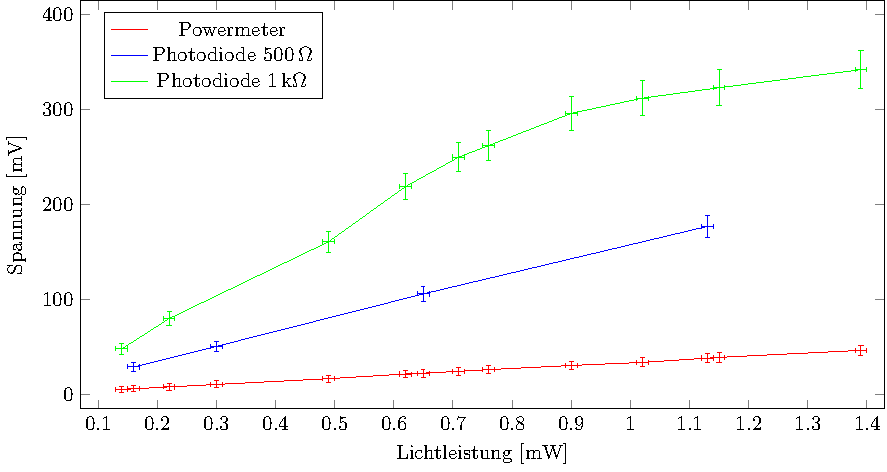
\includegraphics[width=1\linewidth]{graphs/fotodiode/diode.pdf}
	\caption[Vermessung einer Photodiode]{
		Spannungen gemessen über je einen zu einer Photodiode parallel geschalteten Widerstand mit 500 und \unit[1000]{$\Omega$}. Zusätzlich ist der Verlauf der Spannung eines Powermeters aufgetragen.
	}
	\label{fig:photodiode}
\end{figure}

Daher wurde der Aufbau mit kleineren Widerstandswerten von 500 und \unit[1000]{$\Omega$} getestet. Die gemessenen Spannungen sowie die dazu vom Powermeter abgelesenen Werte für die Lichtleistung sind in Abbildung~\ref{fig:photodiode} aufgetragen.

Es ist für \unit[1]{$k\Omega$} eine Sättigung ab etwa \unit[0,9]{mW} erkennbar, die Variante mit \unit[500]{$\Omega$} weist im gesamten Messbereich ein sehr lineares Verhalten auf. Die Fehlerbalken in der x-Achse wurden zu \unit[0,01]{mW} gewählt, da das Powermeter nur zwei Nachkommastellen anzeigt. Der Fehler in der y-Achse wurde auf etwa 5\% gewählt.

%Bei dieser Wellenlänge hat die Photodiode eine Effizienz von etwa \unit[20]{\%} bei der Umwandlung von Licht zu Strom. Bei \unit[660]{nm} (Frequenz des Lasers) etwa \unit[40]{\%}.
